% =====================================================================
%  Sections 1--3: Introduction, Method of Characteristics, Breakdown of
%  classical solutions.
% =====================================================================

\section{Introduction}
\label{sec:motivation}

The viscous Burgers' equation
\begin{equation}
  \label{eq:viscous-burgers}
  u_t + u\,u_x = \nu\,u_{xx}, \qquad \nu>0,
\end{equation}
was introduced by Burgers \cite{burgers1948} as a one-dimensional model of
turbulence; it had appeared earlier in work of Bateman \cite{bateman1915}. It
has the form of the Navier--Stokes momentum equation without the pressure term,
and combines nonlinear advection with viscous diffusion. Setting $\nu=0$ gives
the inviscid equation
\begin{equation}
  \label{eq:inviscid-burgers}
  u_t + u\,u_x = 0,
\end{equation}
the scalar conservation law $u_t+f(u)_x=0$ with flux $f(u)=u^2/2$. Conservation
laws of this type arise in gas dynamics \cite{evans2010,leveque2002} and traffic flow \cite{lighthill1955}.
Burgers' equation is the simplest model in which nonlinearity alone produces
discontinuities: it is the standard test case for shock-capturing numerical
methods, and it is one of the few nonlinear equations that can be solved exactly,
through the Cole--Hopf transformation, so that every claim about shocks and entropy
can be checked against an explicit formula.

Classical solutions of \eqref{eq:inviscid-burgers} can break down in finite time
for smooth data (as soon as $u_0'$ is negative somewhere; see
Section~\ref{sec:shock-formation}), beyond which they can be continued only in
the weak sense, and weak solutions are not unique. Since
\eqref{eq:inviscid-burgers} idealises \eqref{eq:viscous-burgers} for small $\nu$,
with a shock appearing as a layer of thickness $O(\nu)$, the admissible weak
solutions should be those that arise as limits of viscous solutions. We
therefore ask \emph{why the inviscid Burgers' equation requires an entropy
condition, and why that condition is the correct one}. The answer is that the
entropy condition is the criterion selected by vanishing viscosity, a result due
to Hopf (Section~\ref{sec:extensions}). Sections~\ref{sec:characteristics} and
\ref{sec:shock-formation} locate the breakdown of classical solutions, and
Sections~\ref{sec:weak-solutions}--\ref{sec:riemann-problem} develop weak
solutions, their non-uniqueness and the entropy conditions that restore
uniqueness, culminating in the Riemann problem; Section~\ref{sec:extensions}
connects these with the Cole--Hopf formula, vanishing viscosity and Godunov's
method. The theory follows \cite[\S3.4]{evans2010}.

% =====================================================================

\section{Method of Characteristics}
\label{sec:characteristics}

Consider the initial value problem
\begin{equation}
  \label{eq:ivp}
  \begin{cases}
    u_t + u\, u_x = 0, & x \in \mathbb{R},\ t > 0, \\
    u(x,0) = u_0(x), & x \in \mathbb{R},
  \end{cases}
\end{equation}
with $u_0 \in C^1(\mathbb{R})$ in Sections~\ref{sec:characteristics} and
\ref{sec:shock-formation}. For discontinuous data, such as the Riemann data
\eqref{eq:riemann-data}, \eqref{eq:ivp} is understood in the weak sense of
Definition~\ref{def:weak-solution}.

\subsection{Characteristics}
\label{subsec:char-lines}

A \emph{characteristic} of a $C^1$ solution $u$ is a curve $x(t)$ satisfying
\begin{equation}
  \label{eq:char-ode-x}
  \dot{x}(t) = u(x(t), t).
\end{equation}
Along it,
\begin{equation}
  \label{eq:char-ode-u}
  \frac{d}{dt}\, u(x(t), t) = u_x\,\dot{x} + u_t = u_t + u\,u_x = 0 .
\end{equation}

Consequently $u$ is constant along each characteristic, so $\dot x$ is constant:
if $u$ is a $C^1$ solution of \eqref{eq:ivp} on $\mathbb{R}\times[0,T)$ and $x(t)$
solves \eqref{eq:char-ode-x} with $x(0)=x_0$, then for $0\le t<T$
\begin{equation}
  \label{eq:char-formula}
  u(x(t), t) = u_0(x_0), \qquad x(t) = x_0 + u_0(x_0)\, t,
\end{equation}
that is, characteristics are straight lines.

\subsection{The implicit solution formula}
\label{subsec:char-implicit-formula}

\begin{theorem}[Implicit solution via characteristics]
\label{thm:implicit-solution}
Let $u_0 \in C^1(\mathbb{R})$, $\Phi_t(x_0) = x_0 + u_0(x_0)\, t$, and
$T\in(0,\infty]$ such that for every $t\in[0,T)$, $\Phi_t'>0$ on $\mathbb{R}$
and $\Phi_t$ maps $\mathbb{R}$ onto $\mathbb{R}$. Then the function $u$ defined
implicitly by
\begin{equation}
  \label{eq:implicit-solution}
  u(x,t) = u_0(x_0), \qquad \text{where } x = x_0 + u_0(x_0)\, t,
\end{equation}
is the unique $C^1$ solution of \eqref{eq:ivp} on $\mathbb{R}\times[0,T)$.
\end{theorem}

\begin{proof}
\emph{Well-definedness and regularity.} Since $\Phi_t'>0$, $\Phi_t$ is
strictly increasing, hence bijective by hypothesis, so $u(x,t) =
u_0(\Phi_t^{-1}(x))$ is well defined. The function
$F(x_0,x,t)=x_0+u_0(x_0)t-x$ is $C^1$ with $\partial_{x_0}F=\Phi_t'>0$, so by
the implicit function theorem $x_0(x,t)=\Phi_t^{-1}(x)$ is $C^1$ in $(x,t)$
jointly (it is locally the unique root, and by injectivity coincides with the
global one). Hence $u=u_0(x_0(x,t))$ is $C^1$.

\emph{The PDE holds.} Write $x_0 = x_0(x,t) = \Phi_t^{-1}(x)$.
Differentiating $x = x_0 + u_0(x_0)\, t$ in $x$ and in $t$ gives
\begin{equation}
  \frac{\partial x_0}{\partial x} = \frac{1}{1 + u_0'(x_0)\,t},
  \qquad
  \frac{\partial x_0}{\partial t} = \frac{-u_0(x_0)}{1 + u_0'(x_0)\, t},
\end{equation}
both well defined since $\Phi_t'(x_0) = 1+u_0'(x_0)t > 0$. By the chain
rule applied to $u(x,t) = u_0(x_0(x,t))$,
\begin{equation}
  u_x = \frac{u_0'(x_0)}{1 + u_0'(x_0)\,t},
  \qquad
  u_t = \frac{-u_0(x_0)\, u_0'(x_0)}{1 + u_0'(x_0)\, t},
\end{equation}
so $u_t + u\,u_x = 0$, and $u(x,0)=u_0(x)$ since $\Phi_0=\mathrm{id}$.

\emph{Uniqueness.} Let $v$ be any $C^1$ solution of \eqref{eq:ivp} on
$\mathbb{R}\times[0,T)$, and fix $t\in(0,T)$, $x\in\mathbb{R}$. Solve backwards in time
the ODE $\dot\gamma(s)=v(\gamma(s),s)$, $\gamma(t)=x$ (the right-hand side is $C^1$,
hence locally Lipschitz, so there is a unique maximal solution). By
\eqref{eq:char-ode-u}, $v$ is constant along $\gamma$, hence so is $\dot\gamma$:
$\gamma$ is a straight line with bounded slope $v(x,t)$. It therefore stays
bounded and cannot blow up, so it extends back to $s=0$. Setting
$x_0=\gamma(0)$ we get $v(x,t)=v(x_0,0)=u_0(x_0)$ and $x=x_0+u_0(x_0)t$.
Thus every point $(x,t)$ lies on a characteristic coming from $t=0$, with
$x_0=\Phi_t^{-1}(x)$, and $v(x,t)=u_0(\Phi_t^{-1}(x))=u(x,t)$.
\end{proof}

\begin{corollary}[Local existence]
\label{cor:local-existence}
Let $u_0 \in C^1(\mathbb{R})$ with $m := \inf_{x_0} u_0'(x_0) > -\infty$,
and set $T=\infty$ if $m\ge0$ and $T=-1/m$ if $m<0$. Then
\eqref{eq:ivp} has a unique $C^1$ solution on $\mathbb{R}\times[0,T)$,
given by \eqref{eq:implicit-solution}.
\end{corollary}

\begin{proof}
Fix $t\in[0,T)$ and put $\kappa_t := 1+\min(m,0)\,t$, so $\kappa_t>0$ and
$\Phi_t'(x_0)=1+u_0'(x_0)t\ge \kappa_t$ for every $x_0$. Two consequences
follow. (i) $\Phi_t$ is strictly increasing, hence injective. (ii) By the
mean value theorem $\Phi_t(x_0)-\Phi_t(0)\ge \kappa_t x_0$ for $x_0\ge0$ and
$\le \kappa_t x_0$ for $x_0\le0$, so $\Phi_t(x_0)\to\pm\infty$ as
$x_0\to\pm\infty$; by continuity $\Phi_t$ is onto $\mathbb{R}$.
Hence the hypotheses of Theorem~\ref{thm:implicit-solution} hold on
$[0,T)$.
\end{proof}

\begin{remark}
\label{rem:hypothesis-u0prime}
The uniform lower bound $\Phi_t'\ge \kappa_t>0$, not strict monotonicity alone,
gives surjectivity: for $u_0(x)=(\arctan x-x)/t_0$ one has $\Phi_{t_0}(x)=\arctan x$,
strictly increasing with $\Phi_{t_0}'>0$ but not onto $\mathbb{R}$. The
hypothesis $m>-\infty$ cannot be dropped either: for $u_0(x)=x^2$,
$\Phi_t(x)=x+tx^2$ is not injective for any $t>0$, since $\Phi_t'(x)<0$ for
$x<-1/(2t)$.
\end{remark}

% =====================================================================

\section{Breakdown of Classical Solutions}
\label{sec:shock-formation}

\subsection{Blow-up of the derivative and the envelope}
\label{subsec:shock-derivative-blowup}

By the proof of Theorem~\ref{thm:implicit-solution},
\begin{equation}
  \label{eq:ux-formula}
  u_x(x,t) = \frac{u_0'(x_0)}{1 + u_0'(x_0)\, t}, \qquad x = x_0 + u_0(x_0)\, t.
\end{equation}
The formula holds as long as the classical solution exists
(Corollary~\ref{cor:local-existence}, that is, for $t<-1/\inf u_0'$). If
$u_0'(x_0) \geq 0$ the denominator is at least $1$, and $u_x$ remains bounded
along that characteristic. If $u_0'(x_0) < 0$, the right-hand side, regarded as
a formal expression along the characteristic through $x_0$, has a vanishing
denominator at $t = -1/u_0'(x_0)$; the classical solution itself ceases to exist
no later than this time, and strictly earlier unless $x_0$ minimises $u_0'$
(Proposition~\ref{prop:shock-time}). The characteristics
\begin{equation}
  \label{eq:char-family}
  x(x_0, t) = x_0 + u_0(x_0)\, t, \qquad x_0 \in \mathbb{R},
\end{equation}
have an envelope where $\partial x/\partial x_0 = 1 + u_0'(x_0)\,t = 0$, that
is, where $\Phi_t'(x_0)=0$; this concerns the family \eqref{eq:char-family},
not the solution beyond its first breakdown.

\subsection{The breakdown time}
\label{subsec:shock-time}

\begin{proposition}[Breakdown time]
\label{prop:shock-time}
Let $u_0 \in C^1(\mathbb{R})$ with $m := \inf_{x_0} u_0'(x_0)\in(-\infty,0)$, and
set
\begin{equation}
  \label{eq:shock-time}
  T^* = \frac{-1}{m}.
\end{equation}
Then a $C^1$ solution exists on $\mathbb{R} \times [0,T^*)$, with
$\sup_x|u_x(\cdot,t)|\to\infty$ as $t\uparrow T^*$, and for every $T>T^*$ no
$C^1$ solution exists on $\mathbb{R}\times[0,T)$. If the infimum is attained at
$x_0=a$, the solution degenerates at time $T^*$ at the points
\begin{equation}
  \label{eq:shock-location}
  x^* = a + u_0(a)\, T^*, \qquad t^* = T^*.
\end{equation}
\end{proposition}

\begin{proof}
Since $r \mapsto -1/r$ is strictly increasing on $(-\infty,0)$ and
$u_0'(x_0) \geq m$ everywhere, $-1/u_0'(x_0) \geq T^*$ whenever $u_0'(x_0)<0$, so
$\Phi_t'>0$ throughout $[0,T^*)$ and Corollary~\ref{cor:local-existence} gives a
classical solution $u$ there. Choosing $x_n$ with $u_0'(x_n)\to m$,
\eqref{eq:ux-formula} gives $u_x\to m/(1+mt)$ at the point with foot $x_n$, so
$\sup_x|u_x(\cdot,t)|\ge|m|/(1-|m|t)\to\infty$ as $t\uparrow T^*$.

Now let $T>T^*$ and suppose $v$ is a $C^1$ solution on $\mathbb{R}\times[0,T)$.
Since $m<-1/T$, there is $a$ with $u_0'(a)<-1/T$, that is,
$\tau:=-1/u_0'(a)<T$. By \eqref{eq:char-formula} (the characteristic
through $(a',0)$ has bounded slope, hence exists on all of $[0,T)$),
$v(a'+tu_0(a'),t)=u_0(a')$ for every $a'$ and $t<T$. Differentiating in $a'$ at
$a'=a$ gives
\begin{equation*}
  v_x\big(a+tu_0(a),t\big)\,\big(1+t\,u_0'(a)\big)=u_0'(a),
\end{equation*}
and at $t=\tau$ the left side vanishes while the right side is negative, a
contradiction. Finally, if the infimum is attained at $a$, then along the
characteristic from $a$ we have $u_x=m/(1+mt)\to-\infty$ as $t\uparrow T^*$, at
points tending to $(x^*,T^*)$ by \eqref{eq:char-family}.
\end{proof}

\begin{remark}
\label{rem:singularity-vs-shock}
Assume that $u_0$ is bounded, that the infimum $m$ of $u_0'$ is attained, and
that $\{u_0'=m\}$ contains no interval. Then $\Phi_{T^*}'\ge0$ vanishes only on a
set with empty interior, so $\Phi_{T^*}$ is strictly increasing; it is onto
$\mathbb{R}$ because $u_0$ is bounded, so $\Phi_{T^*}(x_0)\to\pm\infty$ as
$x_0\to\pm\infty$ (this replaces the argument of
Corollary~\ref{cor:local-existence}, which degenerates at $t=T^*$). Thus exactly
one characteristic reaches each point at time $T^*$, and $u$, bounded by
$\sup|u_0|$ by \eqref{eq:char-formula}, develops at $(x^*,T^*)$ only a gradient
catastrophe, $|u_x|\to\infty$. If instead $u_0'\equiv m$ on an interval, then
$\Phi_{T^*}$ is constant on it and characteristics carrying different values of
$u_0$ meet at one point at time $T^*$, so one expects a discontinuity to form
at $T^*$; this is not proved here (it follows from the Lax--Oleinik formula,
Remark~\ref{rem:lax-oleinik}).
\end{remark}

\subsection{Example: $u_0=-\arctan x$}
\label{subsec:arctan-breakdown}

Here $u_0'(x_0)=-1/(1+x_0^2)\in[-1,0)$ is minimised at $a=0$ with $m=-1$, so
Proposition~\ref{prop:shock-time} gives $T^*=1$ and $x^*=0$: the singularity
first appears at $(x^*,t^*)=(0,1)$ (Figure~\ref{fig:characteristics}). Here
$\Phi_t'(x_0)=1-t/(1+x_0^2)$ first vanishes at $t=1$, at $x_0=0$. At $t=1$ the
map $\Phi_1(x_0)=x_0-\arctan x_0$ is strictly increasing but its inverse is
not $C^1$ at $0$; for $t>1$, $\Phi_t'<0$ on an interval around $x_0=0$, so
$\Phi_t$ is not injective and characteristics cross.
Geometrically, the characteristic from $x_0$ has speed $u_0(x_0)=-\arctan x_0$, so
those starting near $0$, where $u_0$ falls fastest, converge on one another first,
and the crossing begins at the single point $(0,1)$ rather than everywhere at once.
After that time $u$ would take several values at a point, which is why a notion of
solution that allows jumps is needed.

\begin{figure}[htbp]
\centering
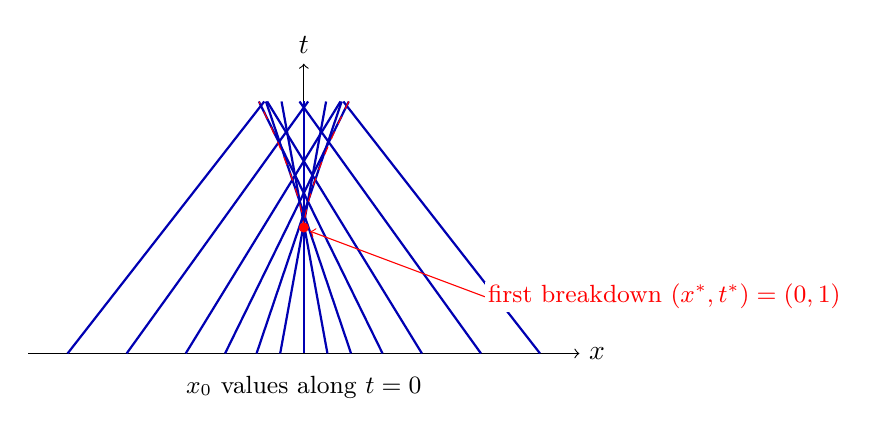
\begin{tikzpicture}[x=1cm,y=1.6cm]
  \draw[->] (-3.5,0) -- (3.5,0) node[right] {$x$};
  \draw[->] (0,0) -- (0,2.3) node[above] {$t$};
  % characteristics x = x0 - arctan(x0) t, drawn for 0 <= t <= 2
  \foreach \xz in {-3,-2.25,-1.5,-1,-0.6,-0.3,0,0.3,0.6,1,1.5,2.25,3}{
    \pgfmathsetmacro{\xe}{\xz - rad(atan(\xz))*2}
    \draw[thick, blue!70!black] (\xz,0) -- (\xe,2);
  }
  % envelope: t = 1+s^2, x = s - arctan(s)(1+s^2)
  \draw[red, dashed, domain=-1:1, samples=40, smooth, variable=\s]
    plot ({\s - rad(atan(\s))*(1+\s*\s)}, {1+\s*\s});
  \filldraw[red] (0,1) circle (1.6pt);
  \draw[red, ->] (2.3,0.45) -- (0.08,0.97);
  \node[red, right, fill=white, inner sep=1pt] at (2.3,0.45) {\small first breakdown $(x^*,t^*)=(0,1)$};
  \node[below] at (0,-0.1) {\small $x_0$ values along $t=0$};
\end{tikzpicture}
\caption{Characteristics $x=x_0-\arctan(x_0)\,t$ for $u_0=-\arctan x$, with
their envelope (red, dashed), which has a cusp at the first breakdown
$(x^*,t^*)=(0,1)$. Inside the cusp ($t>1$) three characteristics pass through
each point.}
\label{fig:characteristics}
\end{figure}

By Remark~\ref{rem:lax-oleinik} and Theorem~\ref{thm:oleinik-uniqueness}, the
entropy solution is given by the Lax--Oleinik formula \eqref{eq:lax-oleinik}.
Here $V(y)=-\big(y\arctan y-\tfrac12\ln(1+y^2)\big)$ is even, and
\begin{equation*}
  \partial_yG(x,y,t)=\frac{\Phi_t(y)-x}{t},\qquad
  \partial_y^2G=\frac{\Phi_t'(y)}{t}=\frac1t-\frac1{1+y^2},\qquad
  \Phi_t(y)=y-t\arctan y .
\end{equation*}

\emph{$t\le1$.} Then $\partial_y^2G>0$ except possibly at $y=0$, so $G(x,\cdot,t)$ is strictly convex and its unique
minimiser is the unique critical point, the characteristic foot $\Phi_t^{-1}(x)$.
Thus the entropy solution is the classical solution
\eqref{eq:implicit-solution}.

\emph{$t>1$.} Now $\Phi_t$ is odd, with $\Phi_t'<0$ exactly on $(-s,s)$,
$s=\sqrt{t-1}$. Fix $x>0$. Since $G(x,y,t)-G(x,-y,t)=-2xy/t$, no minimiser has
$y<0$, and $y=0$ is not one, since $\partial_yG(x,0,t)=-x/t<0$. On $(0,s]$ we
have $\Phi_t\le0<x$, and on $(s,\infty)$ $\Phi_t$ increases from a negative value
to $+\infty$. Hence $G(x,\cdot,t)$ has exactly one critical point
$y_+(x,t)>s$ in $(0,\infty)$, with $\Phi_t'(y_+)>0$; it is the unique
minimiser, and $u=(x-y_+)/t=-\arctan y_+$ is smooth in $x$ by the implicit
function theorem; by oddness the same holds for $x<0$. At $x=0$ the function
$G(0,\cdot,t)$ is even with $\partial_y^2G(0,0,t)=(1-t)/t<0$, so $0$ is not a
minimiser, and the minimisers are $\pm y^*$, where $y^*>0$ is the unique
positive root of $y^*=t\arctan y^*$(the minimum is attained at two symmetric points). Therefore, for $t>1$, the entropy
solution is smooth off $x=0$ and has exactly one jump, stationary at $x=0$ with
\begin{equation*}
  u_\ell=-u_r=\frac{y^*}{t}=\arctan y^*\in(0,\tfrac\pi2).
\end{equation*}
Moreover $y^*=\sqrt{3(1-1/t)}\,(1+o(1))$ as $t\downarrow1$ from
$\arctan y=y-y^3/3+O(y^5)$, so $u_\ell\sim\sqrt{3(t-1)}$, and $y^*>s\to\infty$
gives $u_\ell\to\pi/2$ as $t\to\infty$, matching the limits $u_0(\mp\infty)=\pm\pi/2$.